\chapter{Comparing galaxy morphology and star formation properties in
  X-ray bright and faint groups and cluster}
\label{chap:xray}

\section{Introduction}
\label{sec:intro_x}

Numerous studies have shown a strong environmental dependence on the
star-forming and morphological properties of galaxies
\citep[e.g.][]{butcher1978, dressler1980, postman1984, dressler1999,
  blanton2005b, wetzel2012}.  Low-density regimes tend to be dominated
by star-forming, late-type galaxies whereas high-density areas, such
as galaxy clusters, tend to be primarily populated by quiescent,
early-type galaxies.  Within individual clusters, galaxy morphologies
tend to distribute as a function of local density (or equivalently
cluster-centric radius), with high fractions of late-type galaxies
being found at large radii and the regions near the cluster core being
dominated by early-types \citep[e.g.][]{dressler1980, postman1984,
  postman2005}.  This effect has become known as the
morphology-density relation.  While galaxies tends to distribute based
on their star-forming and morphological properties, the mechanism(s)
responsible for the quenching of star formation and morphological
transformations in galaxies are not well constrained -- although many
have been proposed.  Both mergers and impulsive galaxy-galaxy
interactions (`harassment') \citep[e.g.][]{moore1996} can induce
starburst events in galaxies leading to rapid consumption of gas
reserves and star formation quenching.  Within the virial radius of a
group or cluster the stripping of gas from galaxies becomes
efficient.  Both the stripping of hot halo gas (`strangulation')
\citep[e.g.][]{kawata2008} and cold gas stripping due to a dense
intracluster medium (`ram-pressure') \citep[e.g.][]{gunn1972} can
quench star formation.  As well, tidal interactions can affect gas
reservoirs by transporting gas from the galactic halo outwards which
subsequently allows it to more easily be stripped from the galaxy
\citep{chung2007}.
\par
On top of these environmental quenching mechanisms, previous authors
have found that secular processes, which depend on galaxy mass, appear
to play a significant role in star formation quenching
\citep{balogh2004, muzzin2012}.  The emergent picture for star
formation quenching appears to be some combination of environmental
quenching mechanisms and internal, secular processes.  In particular,
\citep{peng2010} suggests that in the low-redshift Universe,
environmental quenching is dominant for galaxies with $M_\star \lesssim
10^{10.5}\Msun$, whereas for galaxies with $M_\star \gtrsim
10^{10.5}\Msun$ mass quenching plays the more important role.
\par
While environmental and mass quenching within individual haloes are
seemingly strong effects, it is important to realize that groups and
clusters are not isolated structures.  In particular, galaxies can be
pre-quenched in group haloes prior to infall into a larger cluster.
This `pre-processing' suggests that many galaxies may already be
quenched upon cluster infall.  Simulations have shown that between
$\sim 25$ and $45$ per cent of infalling cluster galaxies may have
been pre-processed \citep{mcgee2009, delucia2012}.  Observationally,
\citep{hou2014} find that $\sim 25$ per cent fo the infall population
reside in subhaloes for massive clusters ($M_H \gtrsim 10^{14.5}\Msun$).
This pre-quenching of galaxies in groups could potentially be driven
by galaxy interactions and mergers which are favoured in the group
regime as a result of lower relative velocities between member
galaxies \citep{barnes1985, brough2006}.
\par
An important method for study the quenching mechanisms in groups and
clusters is to study the dependence of the star formation and
morphological properties of galaxies on the conditions of their host
halo (e.g.\ halo mass, X-ray luminosity, etc.).  In particular, if
quenching mechanisms depend on the density of the intra-group/cluster
medium (IGM/ICM) -- for example, ram-pressure stripping of cold gas --
then one would expect to see galaxy populations which are
preferentially passive in haloes with high X-ray luminosities.  Such
correlations have been looked for in previous studies, primarily
within cluster environments.
\par
In particular, \citet{ellingson2001} find no positive correlation
between the fraction of old galaxies and X-ray gas density.
\citet{balogh2002a} conclude that the level of star formation found in
their `low-$L_X$' sample is consistent with the levels seen in their
CNOC1 sample consisting of higher mass clusters.  \citet{fairley2002}
and \citet{wake2005} both study the fractions of blue galaxies at
intermediate redshifts and find no discernible trend between blue
fraction and X-ray luminosity.  Using multivariate regression
\citet{popesso2007b} find that cluster star formation depends on
cluster richness but find no additional dependence on X-ray
luminosity.  In addition, they find no significant correlation between
star-forming fraction and any global cluster property ($M_{200}$,
$\sigma_v$, $N_\mathrm{gal}$, and $L_X$).  \citet{lopes2014} find no
dependence of blue fraction on X-ray luminosity and the only slight
dependence they find between disc fraction and X-ray luminosity is
within the central and most dense regions.
\par
Conversely, \citet{balogh2002b} find that galaxies in their
`low-$L_X$' sample have preferentially high disc fractions compared to
galaxies in their `high-$L_X$' sample.  \citet{postman2005} find that
the bulge-dominated fraction for galaxies in high X-ray luminosity
clusters is higher than for those in low X-ray luminosity clusters.
In contrast with their star formation results, \citet{popesso2007b} do
find a significant anticorrelation between blue fraction and X-ray
luminosity.  Finally, \citet{urquhart2010} find an anticorrelation
between blue fraction and X-ray temperature for galaxies in
intermediate redshift clusters.
\par
In this paper we revisit the dependence of galaxy star formation and
morphological properties on the X-ray luminosity of the host halo.
Specifically, as a result of the large SDSS X-ray sample presented in
\citet{wang2014}, we are able to control for stellar mass, halo mass,
and radial dependences through fine-binning of the data set.  This
allows us to more directly investigate the effect of X-ray luminosity
on galaxies in different environments.
\par
The results of this study are presented as follows.  In
Section~\ref{sec:data_x} we briefly describe the SDSS group catalogues
utilized in this work, as well as the star formation and morphology
catalogues which we match to the group data set.  In
Section~\ref{sec:results_x} we present the primary results of this
paper, specifically, the differences between star-forming and
morphological trends in environments with different X-ray
luminosities.  In Section~\ref{sec:discussion_x} we provide a
discussion of the results presented in this paper.  Finally, in
Section~\ref{sec:conclusions_x} we provide a summary of the key
results and make concluding statements.
\par
In this paper we assume a $\Lambda$ cold dark matter cosmology with
$\Omega_M = 0.3$, $\Omega_\Lambda = 0.7$, and $H_0 = 70\,\mathrm{km}\,\mathrm{s^{-1}}\,\mathrm{Mpc^{-1}}$.

\section{Data}
\label{sec:data_x}

\subsection{Yang group catalogue}

This work relies heavily on the group catalogue of \citet{yang2007}.
The Yang group catalogue is constructed by applying the iterative
halo-based group finder of \citet{yang2005, yang2007} to the New York
University Value-Added Galaxy Catalogue (NYU-VAGC;
\citealt{blanton2005a}), which is based on the Sloan Digital Sky
Survey Data Release 7 (SDSS-DR7; \citealt{abazajian2009}).  The Yang
group catalogue has a wide range of halo masses, spanning from $\sim
10^{12}\Msun$ to $\sim 10^{15}\Msun$.  The catalogue contains both
objects which would be classified as groups ($10^{12} \lesssim M_H
\lesssim 10^{14}$) and as clusters ($M_H \gtrsim 10^{14}\Msun$),
however for brevity we will refer to all systems as groups regardless
of mass.
\par
Groups are initially populated using the traditional
friends-of-friends (FOF) algorithm \citep[e.g.][]{huchra1982}, as well
as assigning galaxies not yet linked to FOF groups as the centres of
potential groups.  Next, the characteristic luminosity, $L_{19.5}$,
defined as the combined luminosity of all group members with
$^{0.1}M_r - 5\log h \le -19.5$, is calculated for each group.  Using
the value of $L_{19.5}$ along with an assumption for the group
mass-to-light ratio, $M_H/L_{19.5}$, a tentative halo mass is assigned
on a group-by-group basis.  The tentative halo mass is used to
calculate a virial radius and velocity dispersion for each group,
which are then used to add or remove galaxies from the system.
Galaxies are assigned to groups under the assumption that the
distribution of galaxies in phase space follows that of dark matter
particles -- the distribution of which is assumed to follow a
spherical NFW profile \citep{navarro1997}.  This process is iterated
until the group memberships no longer change.
\par
Final halo masses given in the Yang group catalogue are determined
using the ranking of the characteristic stellar mass,
$M_{\star,\mathrm{grp}}$, and assuming a relationship between $M_H$
and $M_{\star,\mathrm{grp}}$ \citep{yang2007}.
$M_{\star,\mathrm{grp}}$ is defined by Yang et al. as

\begin{equation}
  M_{\star,\mathrm{grp}} = \frac{1}{g(L_{19.5},\,L_\mathrm{lim})}
  \sum_i \frac{M_{\star,i}}{C_i},
\end{equation}

\noindent
where $M_{\star,i}$ is the stellar mass of the $i$th member galaxy,
$C_i$ is the completeness of the survey at the position of that
galaxy, and $g(L_{19.5},\,L_\mathrm{lim})$ is a correction factor
which accounts for galaxies missed due to the magnitude limit of the
survey.  The statistical error in $M_H$ is on the order of
$0.3\,\mathrm{dex}$ and mostly independent of halo mass
\citep{yang2007}.

\subsection{SDSS X-ray catalogue}

To study the X-ray properties of the group sample, we utilize the SDSS
X-ray catalogue of \citet{wang2014}, which combines ROSAT All Sky
Survey (RASS) X-ray images in conjunction with optical groups
identified from SDSS-DR7 \citep{yang2007} to estimate X-ray
luminosities around $\sim 65\,000$ spectroscopic groups.
\par
To identify X-ray luminosities for individual groups, the algorithm of
\citet{shen2008} is employed.  Beginning from an optical group, the
most massive galaxies (MMGs) of that group are identifed -- up to four
MMGs are kept.  The RASS field in which the MMGs reside are then
identified, and an X-ray source catalogue is generated in the
$0.5-2.0\,\mathrm{keV}$ band \citep{wang2014}.  The maximum X-ray
emission density point is used to identify the X-ray centre of the
group, and any X-ray sources not associated with the group
(e.g.\ point source quasars or stellar object cross-matched from RASS
and SDSS-DR7), within one virial radius , are masked out.  Values for
the X-ray background, centred on the X-ray centre, are determined and
subtracted off and the X-ray luminosity, $L_X$, is calculated by
integrating the source count profile within the X-ray radius.
\par
Determining X-ray luminosities in this manner is susceptible to
`source confusion'.  Due to projection it is possible for more than
one group to contribute to the X-ray emission within the X-ray radius,
leading to an overestimation of the X-ray luminosity for a given
group.  To account for this effect \citet{wang2014} calculate the
`expected' average X-ray flux, $F_{X,i}$, for each group using the
average $L_X - M_H$ relation taken from \citet{mantz2010}.  They then
calculate the sum of the expected fluxes from each group for
multigroup systems and determine the contribution fraction,
$f_{\mathrm{mult},i}$, for each group defined as

\begin{equation}
  f_{\mathrm{mult},i} = F_{X,i} / \Sigma_i F_{X,i}.
\end{equation}

\noindent
The contribution factor will approximate the fraction of the observed
X-ray luminosity intrinsic to the individual group in question,
therefore applying this fraction to each group will act to debias the
measured X-ray luminosity from source confusion contamination.
\par
Within the Wang catalogue 817 groups have $\mathrm{S/N} > 3$, compared
to the total of $34\,522$ groups with positive detections (positive
count rates after background subtraction) and $\mathrm{S/N} > 0$.  We
run our analysis for groups with $\mathrm{S/N} > 3$ as well as groups
with $\mathrm{S/N} > 0$ and find that our choice of signal-to-noise
cut does not change the trends that we observe, therefore we focus on
the total sample ($\mathrm{S/N} > 0$) to ensure a sample size which is
large enough to finely bin the data in various properties
simultaneously.

\subsection{Final data set}

\begin{figure}[!tp]
  \centering
  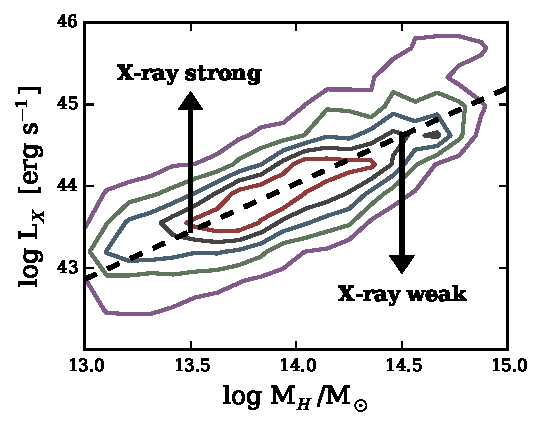
\includegraphics[width=0.8\textwidth]{mh_lx_con.pdf}
  \caption{Density contours for log X-ray luminosity versus log halo
    mass.  Dashed line corresponds to the linear least-squares
    best-fitting relationship.}
  \label{fig:mh_lx_con}
\end{figure}

To obtain the final data set, we match the Wang SDSS X-ray catalogue
to the Yang SDSS group catalogue, giving us both optical and X-ray
group properties for the sample.  To obtain individual galaxy
properties we further match the data set to various public SDSS
catalogues as follows.
\par
We utilize stellar masses given in the NYU-VAGC, which are computed
following the methodology of \citet{blanton2007}.
\par
To obtain star formation rates (SFRs) and specific star formation
rates ($\mathrm{SSFR} = \mathrm{SFR} / M_\star$) we match the
catalogue of \citet{brinchmann2004} to the sample.  SFRs given by
Brinchmann et al. are determined using emission line fluxes whenever
possible; however, in the case of no clear emission lines or
contamination from active galactic nuclei (AGNs), SFRs are determined
using the strength of the $4000\,\mathrm{\mathring{A}}$ break
($D_n4000$) \citep{brinchmann2004}.
\par
We obtain galaxy morphologies from the catalogue of
\citet{simard2011}.  Simard et al. perform two-dimensional bulge +
disc decompositions for over one million galaxies from the Legacy area
of the SDSS-DR7, using three different fitting models: a pure
S{\'e}rsic model, a bulge + disc model with a de Vaucouleurs ($n_b =
4$) bulge, and a bulge + disc model with a free $n_b$.  To distinguish
between discy and elliptical galaxies we utilize the galaxy S{\'e}rsic
index, $n_g$, from the pure S{\'e}rsic decomposition.  We also use the
$V_\mathrm{max}$ weights given by Simard et al. to correct for the
incompleteness of our sample.
\par
We calculate group-centric distances for each galaxy using the
redshift of the group and the angular separation between the galaxy
and the luminosity-weighted centre of its host group.  We normalize
all of the galaxy radii by the virial radius of the host group,
$R_{180}$, which we calculate as in \citet{yang2007}

\begin{equation}
  R_{180} =
  1.26\,h^{-1}\,\mathrm{Mpc}\,\left(\frac{M_H}{10^{14}\,h^{-1}\,\Msun}
  \right )^{1/3} (1 + z_g)^{-1},
\end{equation}

\noindent
where $z_g$ is the redshift of the group centre.

\begin{figure}[!tp]
  \centering
  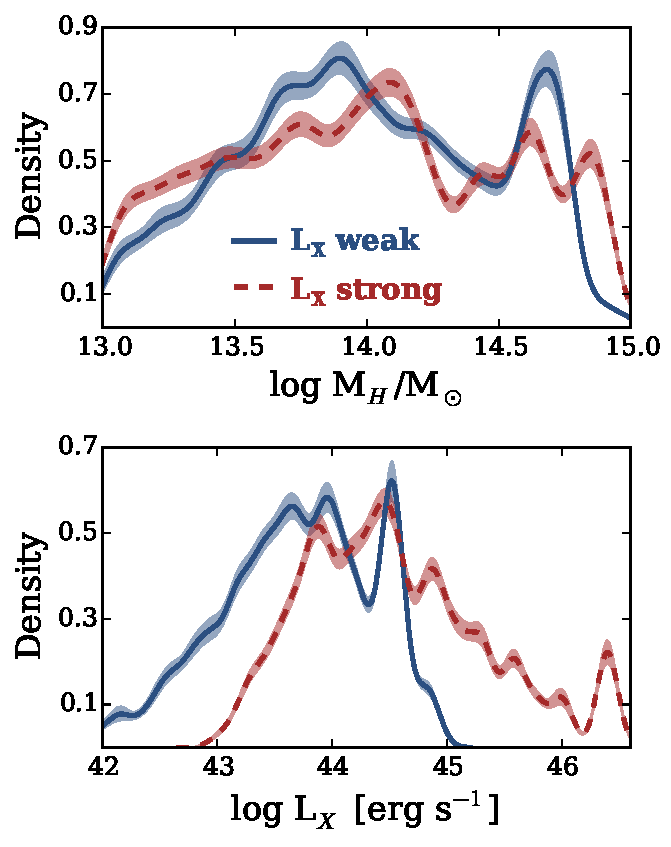
\includegraphics[width=0.8\textwidth]{data_smooth_lx2.pdf}
  \caption{Smoothed distributions for halo mass and X-ray luminosity
    within the sample.  Distributions are shown for both the X-ray
    strong (red, dashed) and the X-ray weak (blue, solid) samples.
    Shaded regions correspond to $2\sigma$ confidence intervals
    obtained from random bootstrap resampling.}
  \label{fig:data_smooth_lx2}
\end{figure} 

The final data set includes groups with halo masses ranging between
$10^{13} - 10^{15}\,\Msun$, and galaxies with stellar masses ranging
from $10^9 - 10^{11.3}\,\Msun$.  Group X-ray luminosities in the data
set are between $10^{39.6} -
10^{46.4}\,\mathrm{erg}\,\mathrm{s^{-1}}$, with a median value of
$10^{43.9}\,\mathrm{erg}\,\mathrm{s^{-1}}$, and are strongly
correlated with halo mass (see Fig.~\ref{fig:mh_lx_con}).  We do not
make an explicit radial cut, however over 99 per cent of member
galaxies fall within 1.5 virial radii.  Our final sample contains
$3\,902$ low-redshift ($z < 0.1$) groups hosting $41\,173$ galaxies.
The catalogue of \citet{wang2014} contains $\sim 35\,000$ groups.  The
fact that the final sample in this work is significantly smaller than
the original catalogue is twofold.  First, we restrict our sample to
redshifts smaller than 0.1 which reduces the number of groups from
$\sim 35\,000$ at $z < 0.2$ to $\sim 18\,000$ at $z < 0.1$.  The
second important cut is that we require $10^{13} < M_H < 10^{15}\Msun$
and a number of groups in the Wang catalogue have halo masses, $M_H <
10^{13}\Msun$ (where halo masses have been obtained from the catalogue
of \citealt{yang2007}).  This cut reduces the remaining number of
groups from $\sim 18\,000$ to $\sim 3\,900$.  It should be noted that
the majority of the $M_H < 10^{13}\Msun$ groups removed from the data
set are groups with very low membership.
\par
To determine the effect of X-ray luminosity on star formation and
morphology we consider two X-ray luminosity samples for the majority
of our analysis, which we refer to as the X-ray weak (XRW) and X-ray
strong (XRS) samples.  Similar to \citet{wang2014}, we define the XRS
sample to consist of all galaxies found below the $\log M_H - \log
L_X$ trend line.  This leads to an approximately equal number of
galaxies within the XRW and XRS samples.  We also performed our
analysis with a cut between the two X-ray samples at the median X-ray
luminosity of the data set, as well as defining the two samples using
the first and the fourth quartiles, however these alternative
definitions of the two X-ray samples do not change the trends that we
observe.
\par
Smoothed distributions for halo mass and X-ray luminosity are shown in
Fig.~\ref{fig:data_smooth_lx2} for both X-ray luminosity samples.
Density distributions are calculated using the \texttt{density}
\{\texttt{stats}\} function in the statistical computing language
\textsc{R} \citep{r2013}\footnote{http://www.R-project.org/} using a
Gaussian kernel.
\par
We study the dependence of star formation rates and morphology on
stellar mass by binning the data by stellar mass and calculating the
disc and star-forming fractions for each bin.  Binning by stellar mass
is important to account for the systematic dependence of star
formation and morphology on stellar mass
\citep[e.g.][]{brinchmann2004, whitaker2012}.  Additionally, as the
relative balance between environmental and mass quenching is not well
understood, it is important to investigate the effects of environment
at a given stellar mass.
\par
We define the star-forming fraction, $f_{SF}$, as the fraction of
galaxies in each bin with $\log \mathrm{SSFR} > -11$.
\citet{wetzel2012} show that at low redshift the division between the
red sequence and the blue cloud is found at $\log \mathrm{SSFR} \simeq
-11$ across a wide range of halo masses.  For each stellar mass bin
the star-forming fraction is given by

\begin{equation}
  f_{SF} =
  \frac{V_\mathrm{max}\;\mathrm{weighted}\;\mathrm{no.}\;\mathrm{of}\;\mathrm{galaxies}\;\mathrm{with}\;\log
    \mathrm{SSFR} >
    -11}{V_\mathrm{max}\;\mathrm{weighted}\;\mathrm{total}\;\mathrm{no.}\;\mathrm{of}\;\mathrm{galaxies}}
\end{equation}

\noindent
Similarly we define the disc fraction, $f_D$, as the fraction of
galaxies in each bin with S{\'e}rsic index, $n < 1.5$.  For each
stellar mass bin this is given by

\begin{equation}
  f_{SF} =
  \frac{V_\mathrm{max}\;\mathrm{weighted}\;\mathrm{no.}\;\mathrm{of}\;\mathrm{galaxies}\;\mathrm{with}\;
    n < 1.5}{V_\mathrm{max}\;\mathrm{weighted}\;\mathrm{total}\;\mathrm{no.}\;\mathrm{of}\;\mathrm{galaxies}}
\end{equation}

\noindent
We also ran our analysis using a dividing cut at S{\'e}rsic indices of
$n=1.0$ and $n=2.0$ to define a disc galaxy, however using these
alternative definitions for a disc galaxy does not alter the trends
that we observe.

\section{Results}
\label{sec:results_x}

\subsection{Star-forming and morphology trends in strong and weak
  $L_X$ samples}

\begin{figure}[!tp]
  \centering
  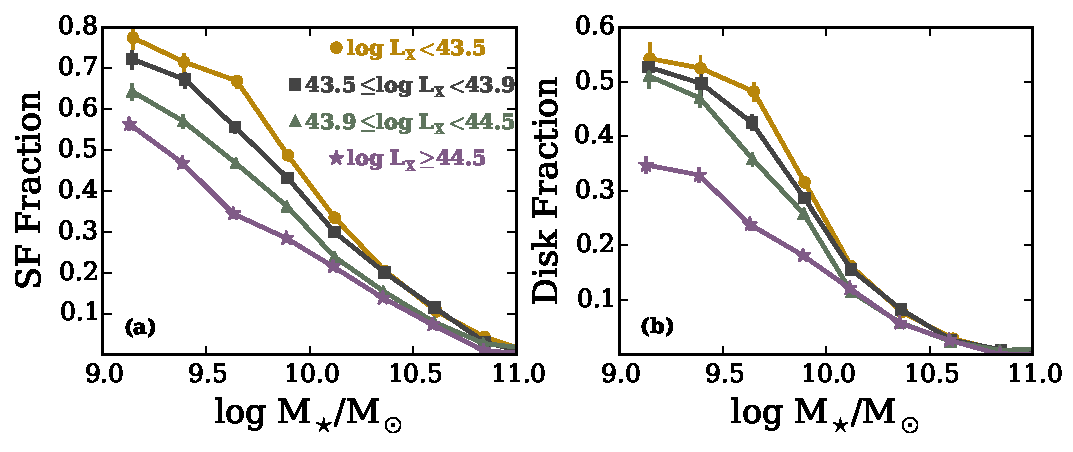
\includegraphics[width=\textwidth]{disk_sfFrac_w_lx1234.pdf}
  \caption{Left: star-forming fraction versus stellar mass for the
    four X-ray luminosity quartiles of the data sample.  Right: disc
    fraction versus stellar mass for the four X-ray luminosity
    quartiles of the sample.  Error bars correspond to $1\sigma$
    Bayesian binomial confidence intervals given in \citet{cameron2011}}
  \label{fig:disk_sfFrac_w_lx1234}
\end{figure}

To investigate the effect of X-ray luminosity on galaxy properties, in
Fig.~\ref{fig:disk_sfFrac_w_lx1234} we show star-forming and disc
fractions, as a function of stellar mass, for subsamples corresponding
to the four X-ray luminosity quartiles of the data set.  Examination
of Figs~\ref{fig:disk_sfFrac_w_lx1234}(a) and (b) show that
star-forming and disc fractions follow a consistent marching order
with respect to X-ray luminosity.  The disc and star-forming fractions
decrease as X-ray luminosity increases.

\begin{figure}[!tp]
  \centering
  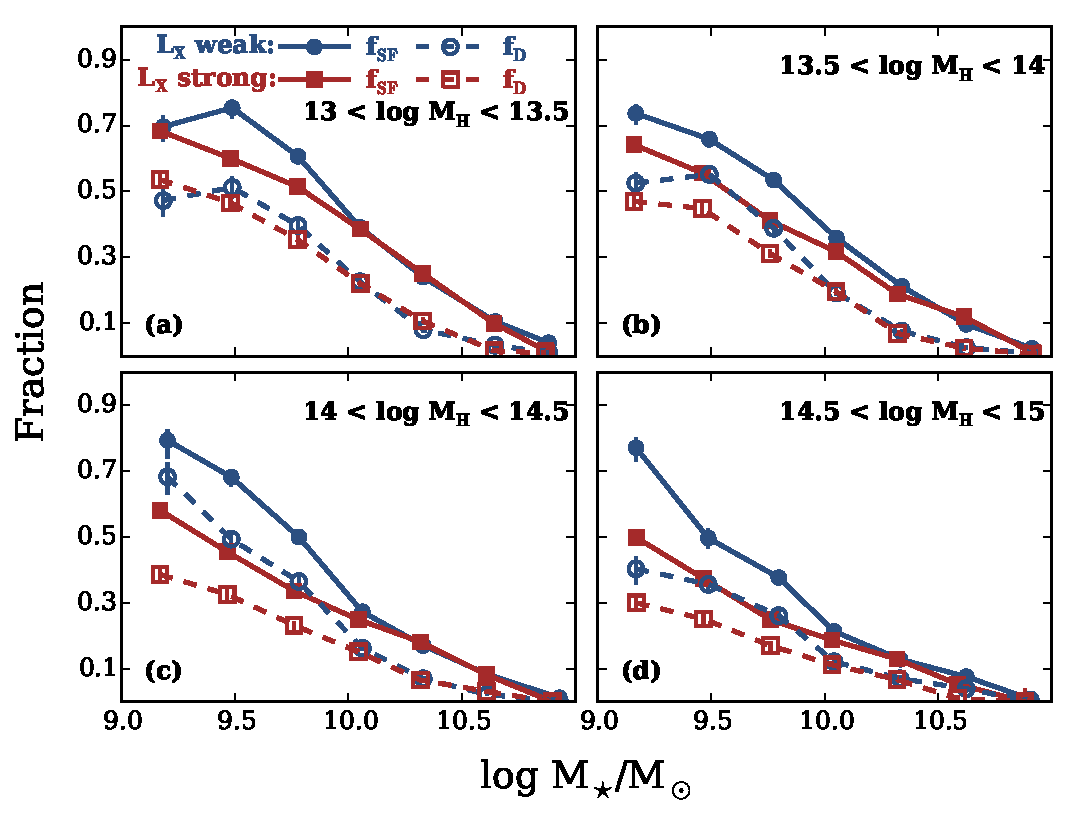
\includegraphics[width=\textwidth]{disk_sfFrac_w_lx2_mh.pdf}
  \caption{Star-forming (solid lines) and disc (dashed lines)
    fractions versus stellar mass, for different halo mass bins and
    the XRW (blue) and XRS (red) samples.  Error bars correspond to
    $1\sigma$ Bayesian binomial confidence intervals given in \citet{cameron2011}}
  \label{fig:disk_sfFrac_w_lx2_mh}
\end{figure}

We note that the results in Fig.~\ref{fig:disk_sfFrac_w_lx1234}
consider all halo masses in the sample, however it has been found that
galaxy morphology and star formation depend on local density and halo
mass \citep{dressler1980, balogh2004, wetzel2012, lackner2013}
(however also see: \citealt{delucia2012, hoyle2012, hou2013}).  As
shown in Fig.~\ref{fig:mh_lx_con} the data show a strong correlation
between X-ray luminosity and halo mass, therefore we must determine if
differences shown in Fig.~\ref{fig:disk_sfFrac_w_lx1234} are simply a
result of galaxies in higher $L_X$ environments being housed in
preferentially high-mass haloes.
\par
To control for any potential halo mass effect, we further bin the data
into narrow halo mass bins and re-examine the dependence of galaxy
properties on X-ray luminosity, considering now the XRW and XRS
samples form Fig.~\ref{fig:mh_lx_con}.
Fig.~\ref{fig:disk_sfFrac_w_lx2_mh} shows star-forming (solid) and
disc (dashed) fractions as a function of stellar mass for four
different halo mass bins -- ranging from $10^{13}$ to $10^{15}\Msun$
with bin widths of $0.5\,\mathrm{dex}$.  Data are binned according to
stellar mass and markers are plotted at the median bin values.  For
each halo mass bin we show star-forming and disc fractions from the
X-ray strong and X-ray weak samples.
\par
For both star-forming and disc fractions we continue to see a residual
trend with X-ray luminosity, even after controlling for any halo mass
dependence: star-forming and disc fractions are systematically higher
in the XRW sample.  We see the strongest trends in the intermediate
and high-mass haloes.  The difference between the strong (red) and
weak (blue) X-ray luminosity samples is clearest at low stellar mass,
and in all haloes the two samples converge at moderate to high stellar
mass.

\subsection{Radial dependence of star-forming and morphology trends}

\begin{figure}[!tp]
  \centering
  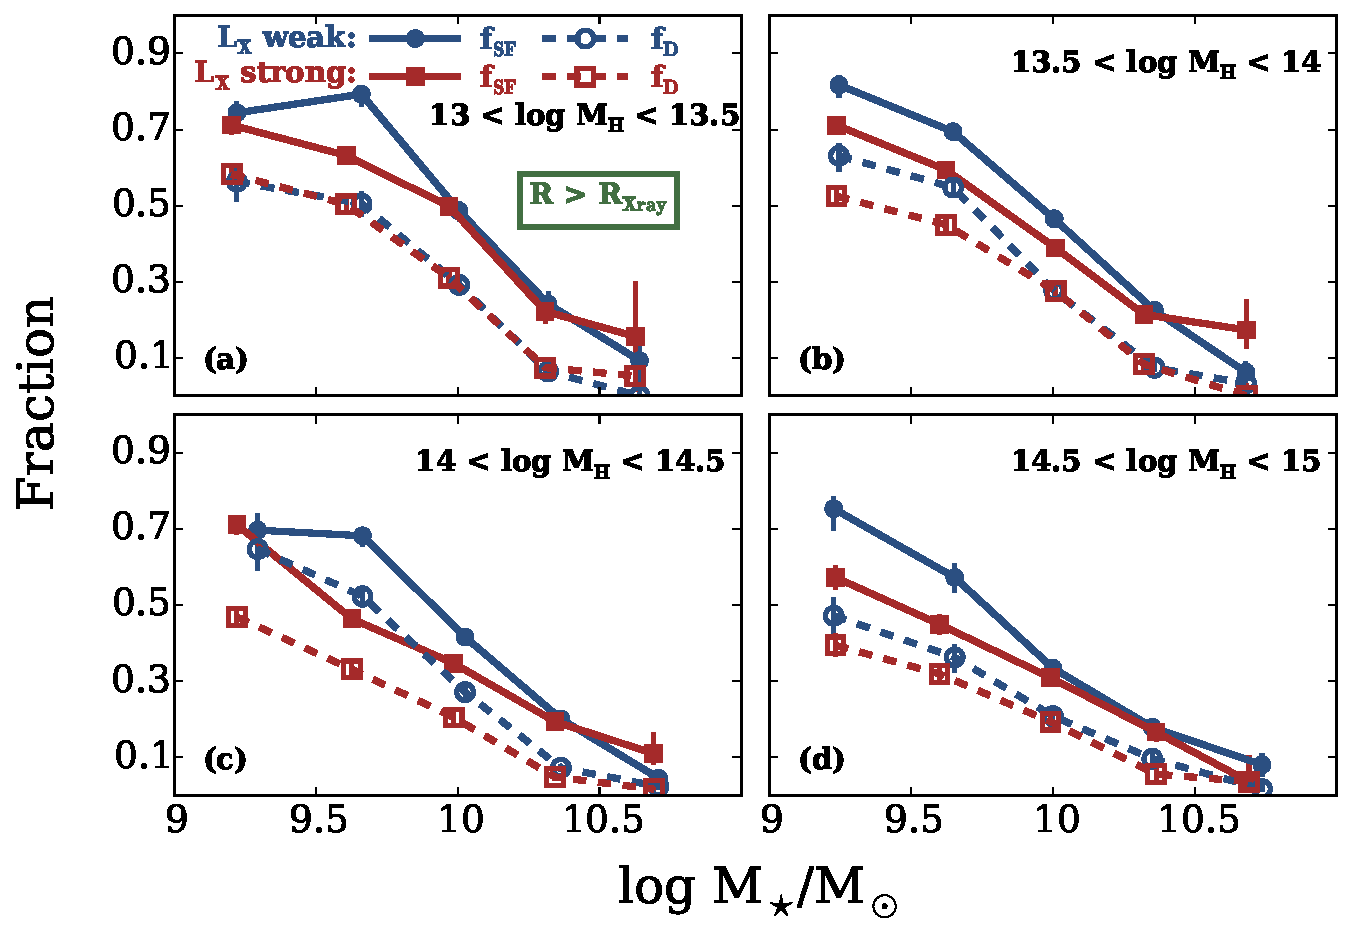
\includegraphics[width=\textwidth]{disk_sfFrac_w_lx2_mh_rxh.pdf}
  \caption{Star-forming (solid lines) and disc (dashed lines)
    fractions versus stellar mass, for galaxies outside of their host
    X-ray radius and for different halo mass bins and
    the two $L_X$ samples.  Error bars correspond to
    $1\sigma$ Bayesian binomial confidence intervals given in \citet{cameron2011}}
  \label{fig:disk_sfFrac_w_lx2_mh_rxh}
\end{figure}

\begin{figure}[!tp]
  \centering
  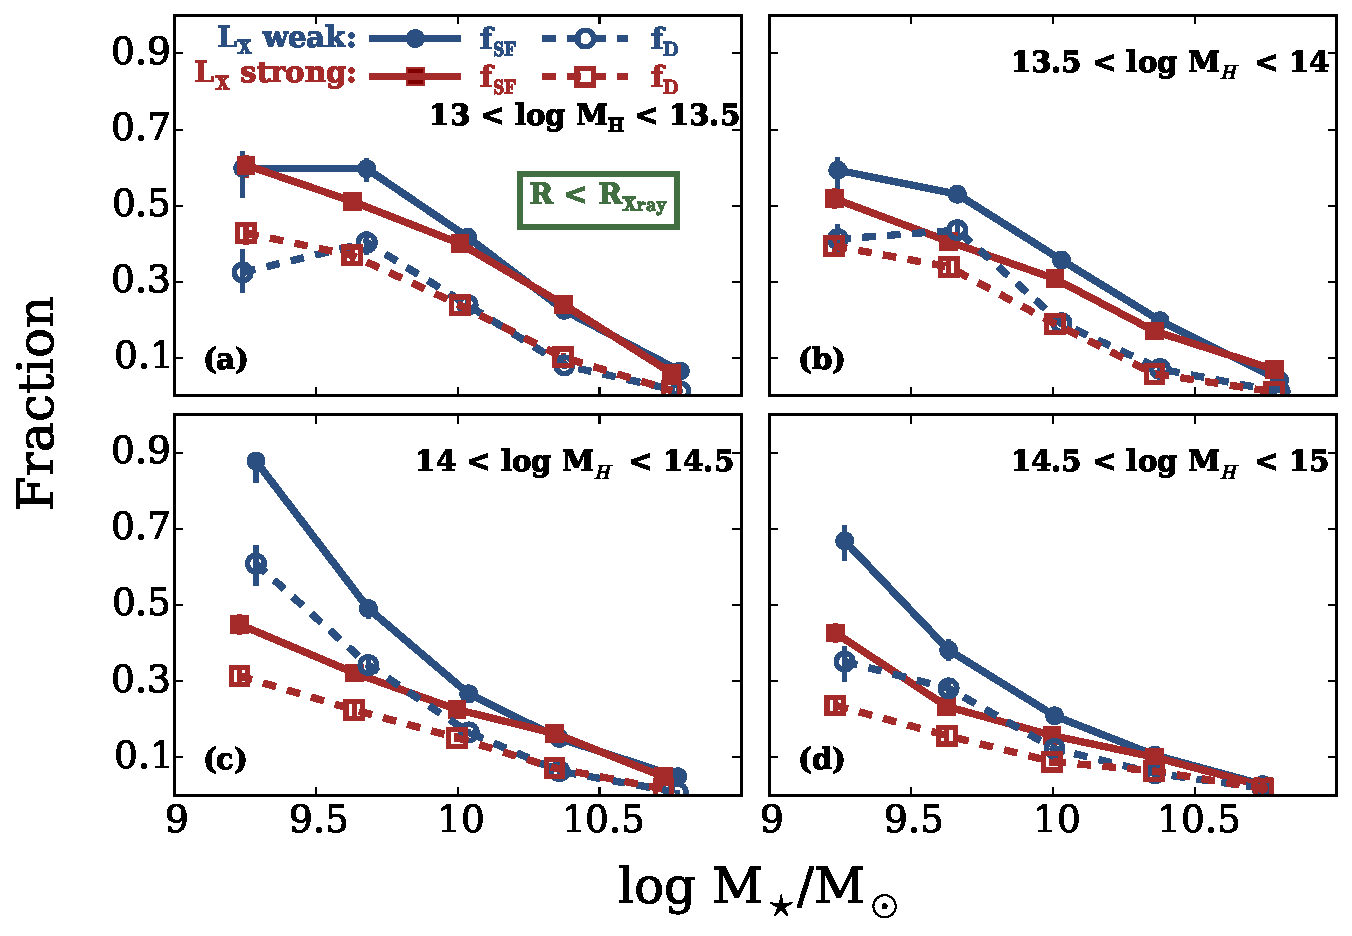
\includegraphics[width=\textwidth]{disk_sfFrac_w_lx2_mh_rxl.pdf}
  \caption{Same as Fig.~\ref{fig:disk_sfFrac_w_lx2_mh_rxh} for
    galaxies inside of their host X-ray radius.}
  \label{fig:disk_sfFrac_w_lx2_mh_rxl}
\end{figure}

Within host groups X-ray emission is concentrated at relatively small
group-centric radii, with X-ray emission generally extending out to
half a virial radius \citep{wang2014}.  If the trends we are observing
are a result of increased gas density, we would expect to see enhanced
trends (i.e.\ a larger difference between the XRS and XRW samples) at
small group-centric radii and suppressed trends at large radii.  To
test this we further divide the data into subsets corresponding to
those galaxies that lie within the X-ray emission radius (using the
X-ray radius, $R_\mathrm{Xray}$, given in \citealt{wang2014}) and
those galaxies that lie outside of the X-ray radius.  We again plot
star-forming/disc fraction versus stellar mass, in narrow halo mass
bins, for the large and small radius subsamples.  The results of this
analysis are shown in Figs~\ref{fig:disk_sfFrac_w_lx2_mh_rxh} and
\ref{fig:disk_sfFrac_w_lx2_mh_rxl}, where the two figures correspond
to disc fraction and star-forming fraction trends for the large and
small radius subsamples, respectively.
\par
Examination of Figs~\ref{fig:disk_sfFrac_w_lx2_mh_rxh} and
\ref{fig:disk_sfFrac_w_lx2_mh_rxl} shows that for both galaxies found
within their host halo's X-ray radius and those found outside, we
still see an increase in star-forming and disc fractions in the XRW
sample -- as before this effect is strongest in the intermediate-to
high-mass haloes and at low stellar mass.  Also the disc and
star-forming fractions tend to be higher at large radii, which is
consistent with the morphology-density relation.

\begin{figure}[!tp]
  \centering
  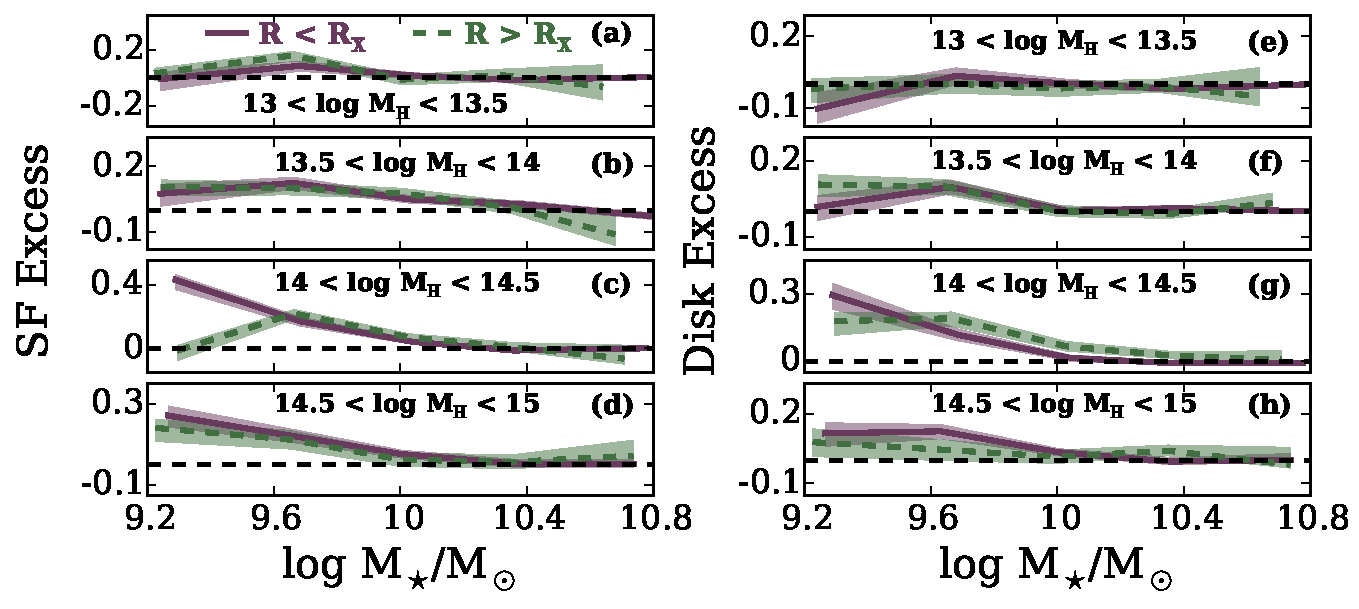
\includegraphics[width=\textwidth]{lxDiff_r.pdf}
  \caption{SF and disc excess versus stellar mass for both galaxies
    within (purple, solid) and outside (green, dashed) of the X-ray
    radius.  Panels a-d show SF excess for four halo mass bins and
    panels e-h show disc excess for four halo mass bins.  Shaded
    regions represent $1\sigma$ confidence intervals.}
  \label{fig:lxDiff_r}
\end{figure}

To further investigate if the increase in star-forming and disc
fractions in the XRW sample compared to the XRS sample -- which we
will refer to as the `SF excess' and the `disc excess' -- depends on
whether you consider galaxies within or outside of the X-ray radius,
we show SF and disc excess versus stellar mass in
Fig.~\ref{fig:lxDiff_r}.  We quantitatively define SF and disc excess
as

\begin{align}
  & \mathrm{SF}\;\mathrm{excess} = f_{SF}(\mathrm{XRW}) -
  f_{SF}(\mathrm{XRS}) \label{eq:f_sf} \\
  & \mathrm{Disc}\;\mathrm{excess} = f_{D}(\mathrm{XRW}) -
  f_{D}(\mathrm{XRS}) \label{eq:f_d}
\end{align}

\noindent
where $f_{SF}(\mathrm{XRW})$ and $f_{SF}(\mathrm{XRS})$ are the
star-forming fractions in the XRW and XRS samples respectively, and
analogously for $f_D(\mathrm{XRW})$ and $f_D(\mathrm{XRS})$.
\par
We find no radial dependence for SF and disc excess as the two radial
subsamples in Fig.~\ref{fig:lxDiff_r} show overlap for all halo and
stellar masses.  With the exception in Fig.~\ref{fig:lxDiff_r}(c) where
the SF excess, for low-mass galaxies, is stronger for galaxies within
the X-ray radius. 

\section{Discussion}
\label{sec:discussion_x}

\begin{figure}[!tp]
  \centering
  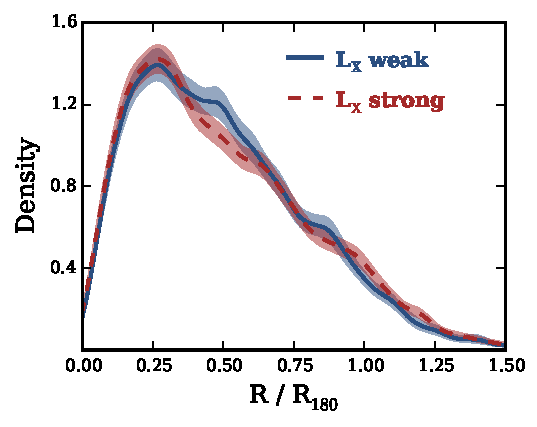
\includegraphics[width=0.8\textwidth]{r_smooth_lx2.pdf}
  \caption{Smoothed radial distributions of galaxies in the XRW (blue,
  solid) and XRS (red, dashed) samples.  Shaded regions correspond to
  $2\sigma$ confidence intervals obtained from random bootstrap resampling.}
  \label{fig:r_smooth_lx2}
\end{figure}

We find that star-forming and disc fractions are systematically lower
in the XRS sample than galaxies in XRW environments.  This trend
persists even upon controlling for any halo mass dependence, however
the observed difference between the XRS and the XRW sample is not
enhanced when considering only those galaxies within the X-ray radius
of the host halo.
\par
There are two major observed effects which have been found to impact
the distributions of early-type and late-type galaxies within cluster
environments.  The so called `Butcher-Oemler' (BO) effect is the
observational trend that the blue fraction of cluster galaxies are
positively correlated with redshift \citep[e.g.][]{butcher1984,
  ellingson2001, loh2008, urquhart2010}.  However, it should be noted
that there is still debate when it comes to the physical nature of the
BO effect (for example, see: \citealt{andreon1999, andreon2004,
  andreon2006}.  Since we are only considering low-redshift ($z <
0.1$) galaxies the BO effect should be negligible.
\par
The second major effect is the previously mentioned morphology-density
relationship.  In order to determine if the morphology-density
relation is affecting the trends we observe, we must check if there
are significant differences in the radial distributions of the XRS and
the XRW samples.  For instance, if the XRW sample is found at
systematically high group-centric radii compared to the XRS sample,
then the morphology-density relation could explain why we find
systematically larger star-forming and disc fractions in the XRW
sample.  In Fig.~\ref{fig:r_smooth_lx2} we plot the smoothed radial
distributions for both the XRS and the XRW samples.  We see no
systematic difference between the two distributions, in fact they are
nearly indistinguishable from one another, and therefore any observed
differences betwee the XRS and XRW samples are not being driven by
difffering radial distributions.

\subsection{AGN contamination}

\begin{figure}[!tp]
  \centering
  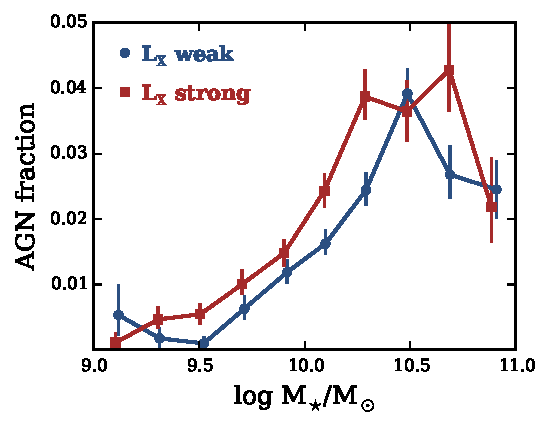
\includegraphics[width=0.8\textwidth]{AGNFrac_w_lx2.pdf}
  \caption{BPT identified AGN fraction versus stellar mass for the XRW
  and XRS samples.  Error bars correspond to $1\sigma$ Bayesian
  binomial confidence intervals given in \citet{cameron2011}.}
  \label{fig:AGNFrac_w_lx2}
\end{figure}

When considering X-ray properties of galaxy groups it is important to
ensure that the observed X-ray emission is due to the hot IGM and not
due to contamination from AGN or other X-ray sources.  In
\citet{wang2014} bright point sources, such as stars and quasars, are
masked out, however it is still important to ensure that our results
are not being contaminated by galaxies housing non-point source AGN.
\par
In Fig.~\ref{fig:AGNFrac_w_lx2} we plot AGN fraction versus stellar
mass for the XRW and XRS samples.  We use AGN classified by
\citet{kauffmann2003}, which are identified using the location of
galaxies on the BPT diagram \citep{baldwin1981}.  I should be noted
that \citet{trouille2010} show that between 20 and 50 per cent
(depending on the dividing line between AGN and star-forming galaxies
used) of X-ray identified AGN fail to be classified as AGN on the BPT
diagram.
\par
We see that the AGN fraction tends to be larger within the XRS sample,
however at all stellar masses the number of AGN galaxies is a modest
fraction (less than 5 per cent) of the total sample, for both XRS and
XRW galaxies.  Most relevant is the fact that at low stellar mass the
AGN fraction is consistently below one per cent, for both the XRW and
XRS samples, whereas the trends we observe with X-ray luminosity are
exclusively seen at low stellar mass
(e.g.\ Fig.~\ref{fig:disk_sfFrac_w_lx2_mh}).  We examined disc and
star-forming fractions for a subsample of the data with galaxies
identified as AGN removed and found that removing AGN galaxies from
the sample does not change the observed trends.  Furthermore, we
examined trends after removing all groups that house galaxies
identified as AGN and again found no change in the observed trends.
Therefore we conclude that AGN are not a significant contributor to
the observed trends in star-forming and disc fractions.

\subsection{Implications for star formation quenching}

\begin{figure}[!tp]
  \centering
  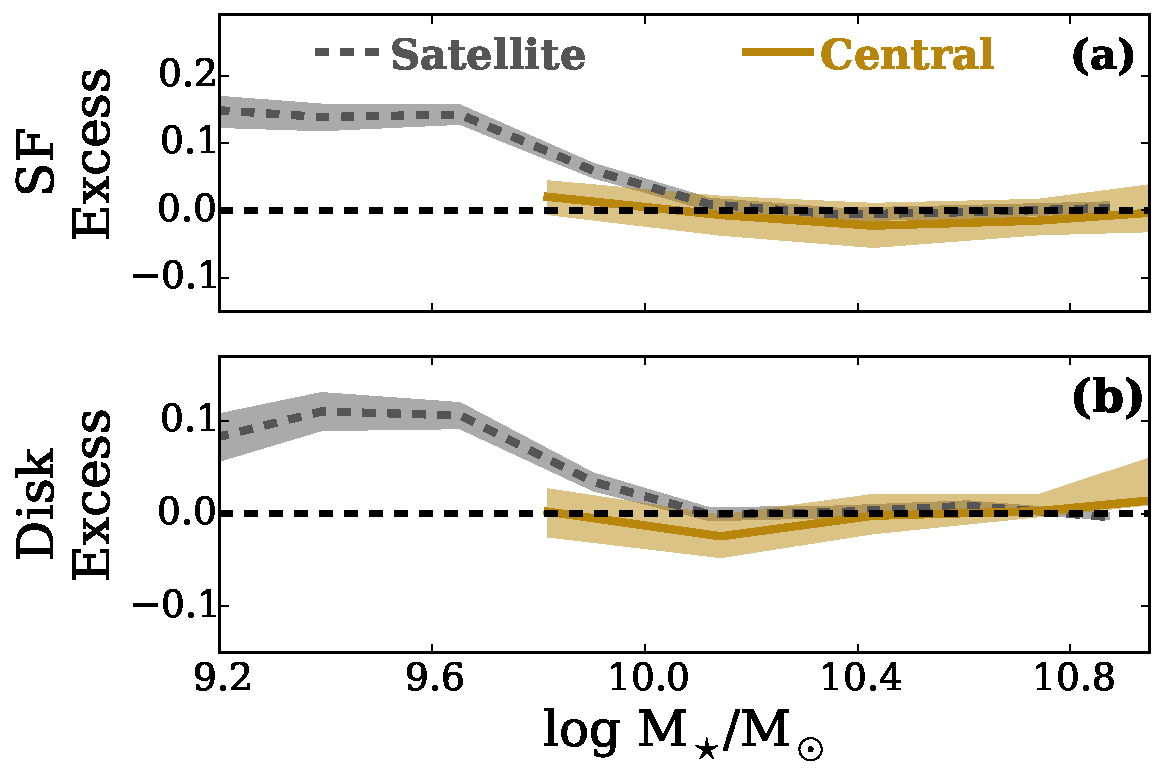
\includegraphics[width=\textwidth]{lxDiff_cs.pdf}
  \caption{SF and disc excess versus stellar mass for both centrals
    (gold, solid) and satellites (grey, dashed).  Shaded regions
    correspond to $1\sigma$ confidence intervals.}
  \label{fig:lxDiff_cs}
\end{figure}

Tje relative importance of various galaxy quenching mechanisms is an
important, open question.  Galaxy populations in groups can be
classified as either `central' (located at the centre of the group
dark matter halo) or `satellite' galaxies.  These two populations are
expected to evolve differently \citep[e.g.][]{vandenbosch2008b}, and
therefore when attempting to elucidate information on the quenching of
galaxies it is important to consider centrals and satellites as
distinct populations.  In Fig.~\ref{fig:lxDiff_cs} we plot SF and disc
excess (equations~\ref{eq:f_sf} and \ref{eq:f_d}) versus stellar mass,
considering separately central and satellite galaxies.  Central
galaxies are defined as the most massive group galaxies and satellite
galaxies are defined as all galaxies which have not been classified as
centrals.
\par
When considering satellite galaxies in Fig.~\ref{fig:lxDiff_cs}(a) we
find that galaxies within the XRW sample have consistently larger
star-forming fractoins at low stellar mass
($\mathrm{SF}\;\mathrm{excess} > 0$), while at large stellar mass the
XRW and XRS samples are indistinguishable.  When considering only
central galaxies we find that there is no difference between the XRW
and XRS samples ($\mathrm{SF}\;\mathrm{excess} \approx 0$) when
considering star-forming fraction.  We observe qualitatively similar
trends for disc excess in Fig.~\ref{fig:lxDiff_cs}(b).  This implies
that whatever effect X-ray luminosity has on star-forming and
morphological properties it only affects satellite galaxies, central
galaxies are insensitive to the group X-ray properties.  This is not
surprising given that central galaxies are massive, and we see no
difference between the XRS and XRW at large stellar mass.
\par
One interpretation of the differences we observe between the XRW and
XRS samples would be to invoke the ram-pressure stripping of satellite
galaxies.  The rate at which galaxies will lose gas through
ram-pressure stripping will increase in proportion to $L_X$
\citep{fairley2002}.  Therefore if ram-pressure is an important
mechanism when it comes to the quenching of galaxies, a decrease in
star-forming fraction should be observed with increasing X-ray
luminosity.  It should be noted that although we observe very similar
trends for star-forming and disc fractions, it is not clear whether
ram-pressure stripping can efficiently drive galaxy morphology
transformations from late to early type \citep{christlein2004}.  Prior
studies \citep[e.g.][]{gavazzi2003, kenney2004, muzzin2014} have found
evidence of ram-pressure stripping.  We note as well that other
studies \citep[e.g.][]{balogh2002a, fairley2002, wake2005, lopes2014}
have found no clear trend between star-forming or blue fractions and
X-ray luminosity.  At first glance the results shown in
Fig.~\ref{fig:disk_sfFrac_w_lx2_mh} are consistent with ram-pressure
stripping; at low stellar masses there are lower star-forming
fractions in the XRS sample.  One difference between the results we
observe and previous studies is that we narrowly bin our data in
stellar mass.  Since star-forming and morphological properties depend
strongly on stellar mass, any residual dependence on X-ray luminosity
may be lost without controlling for stellar mass.  In addition our
sample size is significantly larger than most previous studies, so it
may be that trends with X-ray luminosity are subtle enough to be
missed without large statistics.

\begin{figure}[!tp]
  \centering
  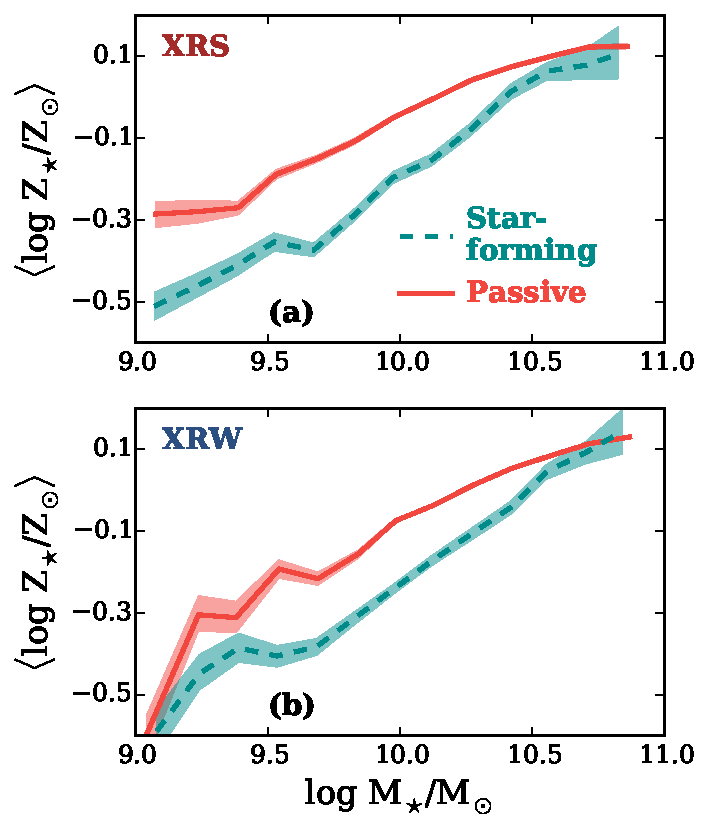
\includegraphics[width=0.8\textwidth]{met_m.pdf}
  \caption{Mean stellar metallicity versus stellar mass for
    star-forming (blue, dashed) and passive (red, solid) galaxies,
    divided by galaxies in the XRS (top) and XRW (bottom) samples.
    Shaded regions correspond to $1\sigma$ confidence intervals
    obtained from random bootstrap resampling.}
  \label{fig:met_m}
\end{figure}

If the trends we detect are driven by ram-pressure we would expect a
radial dependence of our trends with X-ray luminosity.  The efficiency
of ram-pressure stripping is proportional to $\rho v^2$
\citep{wake2005, popesso2007b}, where $\rho$ is the IGM density and
$v$ is the speed of the member galaxies.  Since the IGM density is
highest at small group-centric radii, the efficiency of ram-pressure
stripping should increase towards small radii.  In
Fig.~\ref{fig:lxDiff_r} we showed that the observed SF excess does not
strongly depend on radius.  We conclude that this lack of radial
dependence is inconsistent with the ram-pressure stripping scenario.
\par
Another often-envoked mechanism for regulating star formation is
`galaxy strangulation' \citep{larson1980, balogh2000, kawata2008,
  peng2015}.  Strangulation is a mechanism in which the replenishment
of cold gas on to galaxies is halted, which in turn leads to galaxy
quenching once the galaxy has exhausted its existing cold gas
reservoirs.  The time-scales over which a galaxy will be quenched by
strangulation are longer than the times associated with the direct
stripping of cold gas reserves (ram-pressure).  Recently,
\citet{peng2015} have argued that it is possible to differentiate
between strangulation and direct stripping using metallicity
differences between star-forming and quiescent galaxy populations.  We
direct the reader to \citet{peng2015} for a more complete discussion,
however the main idea is that quenching by strangulation will result
in higher metallicities for passive galaxies compared to star-forming
galaxies.  This is a result of star formation continuing even after
the gas supply has been halted which will increase stellar metallicity
until the cold gas reserves have been exhausted and the galaxy has
therefore been quenched.  This trend in metallicity is not expected
from direct stripping, where star formation shuts off quickly after
the removal of cold gas.
\par
To investigate the effect of strangulation on the galaxy sample in
this study we follow \citet{peng2015} and calculate mean stellar
metallicity versus stellar mass considering star-forming and passive
galaxies separately, for galaxies within our XRW sample as wel as our
XRS sample.  Metallicities are matched to our sample from the
catalogue of \citet{gallazzi2005}, and mean metallicities are
calculated in stellar mass bins with widths of $0.15\,\mathrm{dex}$.
Not all of the galaxies within this sample have measured
metallicities, and our XRW and XRS samples are reduced to $10\,939$
(52 per cent of total sample) and $8\,851$ (44 per cent of total
sample) member galaxies respectively.
\par
In Fig.~\ref{fig:met_m} we see higher stellar metallicities for
passive galaxies compared to star-formers, which we interpret as
evidence for strangulation playing a significant role in star
formation quenching.  Of particular interest for this work is the
behaviour at low stellar mass which is where the dependence of star
formation and morphology on X-ray luminosity is observed (see
Fig.~\ref{fig:disk_sfFrac_w_lx2_mh}).  We see a somewhat stronger
strangulation signal (ie.\ difference between passive and star-former
metallicity) for galaxies in the XRS sample compared to the XRW
sample, at low stellar mass.
\par
In light of this observed difference, it is important to note that
compiling this subsample of galaxies with measured metallicities does
not affect all stellar masses equally.  Specifically, low-mass
galaxies are preferentially removed from the sample when matching to
the metallicity catalogue.  In particular, 69 per cent of low-mass
($M_\star < 10^{9.5}\Msun$) galaxies in the XRS sample do not have
measured metallicities, whereas in the XRW sample 75 per cent of
low-mass galaxies do not ahve measured metallicities.  Not only are
low-mass galaxies being preferentially lost, but the fraction of
low-mass galaxies being lost is slightly different between the two
X-ray samples.  Therefore, although the results in
Fig.~\ref{fig:met_m} are consistent with strangulation -- and more
specifically, somewhat stronger strangulation at the low-mass end of
the XRS sample -- we suggest that this trend be interpreted with
caution as completeness differences could be playing some role.

\subsection{Group evolutionary/dynamical state}

The dynamical state of galaxy groups is an important evolutionary
indicator and can potentially influence galaxy properties.  Trends
with X-ray luminosity may reflect that the XRW and XRS samples have
different dynamical properties as it is expected that more evolved
groups with relaxed dynamics would be more X-ray luminous
\citep{popesso2007a}.
\par
Theoretically the velocity distribution of galaxies within a group in
dynamical equilibrium should have a characteristic Gaussian shape.
Groups lacking this Gaussian distribution can therefore be considered
as being unevolved, dynamically young systems.  To investigate the
dependence on the dynamical state of the groups in our data set we
follow the procedure of \citet{hou2009} and apply the Anderson-Darling
normality (ADN) test to the velocity distributions of the galaxies in
the group sample.  The ADN test is a non-parametric test which
compares the cumulative distribution function (CDF) of the data to the
CDF of a normal distribution to determine the probability (p-value)
that the difference between the distribution of the data and that of a
Gaussian is as large as observed (or larger), under the assumption
that the data is in fact normally distributed.  For our dynamical
analysis we use a subset of the data consisting of only those groups
with eight or more members ($31\,820$ galaxies in $1\,456$ groups), in
order to ensure reasonable statistics when applying the ADN test.  To
obtain values for the ADN statistic for each of our groups we employ
the \texttt{ad.test \{nortest}\} function in the statistical computing
language \textsc{R} \citep{r2013} -- large values of the ADN statistic
are indicative of less Gaussian distributions.
\par
Initially, we examine the dynamical states of galaxies within the XRW
and XRS samples globally (ie.\ no radial cuts) and we find no
systematic differences between the dynamical states of XRW and XRS
galaxies.  \citet{popesso2007a} study the difference between X-ray
underluminous Abell (AXU) clusters and normal Abell clusters.  They
find that while both AXU and normal Abell clusters show Gaussian
velocity distributions within the virialized region ($R <
1.5\,\mathrm{R_{200}}$), within the exterior regions ($1.5 \le R \le
3.5\,\mathrm{r_{200}}$) the AXU cluster show sharply peaked,
non-Gaussian velocity distributions.  The authors interpret these
leptokurtic velocity distributions in the outer cluster regions as
evidence that AXU clusters have experienced recent accretion/merging.
If the XRW groups have experienced more recent accretion of galaxies
from the field and smaller groups than the XRS groups, then this could
contribute to the dependence we observe between star-forming and disc
fractions on X-ray luminosity.  Galaxies in underdense regions (the
field, low-mass groups) have been found to be preferentially star-
forming with late-type morphologies.  Accordingly, groups experiencing
recent accretion may contain more star-forming, late-type, galaxies
when compared to groups which are dynamically older.
\par
To investigate this possibility we study the dynamical states of
groups in both the XRW and XRS samples, and divide member galaxies
into two radial subsamples: those found in the inner regions ($R <
R_{180}$) of their host group, and those found in the outer regions
($R \ge R_{180}$) of their host group.  This is similar to the
analysis performed by \citet{popesso2007a}.  Instead of making an
arbitrary, discrete cut to define Gaussian and non-Gaussian groups we
treat the AD statistic values as continuous and compare the
distributions of ADN statistics from the four subsamples (XRW inner,
XRW outer, XRS inner, XRS outer) to determine whether there are any
significant differences in dynamical state.  To quantitatively compare
the distributions we utilize the two-sample Anderson-Darling (AD2)
test.  The AD2 test is similar to the ADN test, however instead of
comparing observed data to the normal distribution, it compares the
CDFs of two data samples to determine whether they are drawn from the
same underlying distribution.  We apply the AD2 test to the
distributions of ADN statistic values for the XRW and XRS samples to
determine if the dynamical states vary between the inner and the outer
regions.  To perform the AD2 test between the subsamples we use the
\texttt{ad.test \{kSamples\}} function in the statistical computing
language \textsc{R} \citep{r2013}.
\par
We find no evidence ($\mathrm{p-value} = 0.38$) for different
dynamical states in the inner and outer regions of the XRS sample,
however for the XRW sample we find strong evidence ($\mathrm{p-value}
= 3 \times 10^{-7}$) that the dynamical state of galaxies in the outer
region is different from those in the inner region.  When we examine
the distributions of ADN statistics for the four subsamples we find
that the ADN statistic values for the XRW outer subsample are
systematically higher than for the other three subsamples.  This
suggests that the velocity distributions for galaxies outside of the
virial radius in the XRW sample are less Gaussian than the rest of the
data set.
\par
This result is consistent with \citet{popesso2007a}, who find
non-Gaussian velocity distributions for galaxies in the outer regions
of X-ray underluminous Abell clusters.  This result supports the
notion that the increased number of star-forming and late-type
galaxies we observe in the XRW sample can potentially be explained by
underluminous X-ray groups experiencing recent accretion of field
galaxies and small galaxy groups, as this recent accretion can give
rise to less Gaussian velocity distributions in the exteriors of these
groups.
\par
We do note that it remains difficult to simultaneously explain the
dynamical results together with the fact that we observe no dependence
of SF and disc excess on radius (Fig.~\ref{fig:lxDiff_r}).

\section{Summary \& Conclusions}
\label{sec:conclusions_x}

We have used a sample of galaxies taken from X-ray emitting groups and
clusters in the SDSS to study the effect of X-ray luminosity on galaxy
star formation and morphological properties.  Using a data set
spanning a large range in stellar mass ($10^9 - 10^{11.3}\Msun$), halo
mass ($10^{13} - 10^{15}\Msun$), and X-ray luminosity ($10^{39.6} -
10^{46.4}\mathrm{erg}\,\mathrm{s^{-1}}$) we have investigated the
differences between disc and star-forming fractions within different
X-ray environments.  The main results of this paper are as follows.

\begin{enumerate}[(i)]
  \item Star-forming and disc fractions are preferentially lower
    within the X-ray strong sample when compared to galaxies within
    the X-ray weak sample -- this trend remains after controlling for
    any halo mass dependence.

  \item This difference between the X-ray strong and X-ray weak
    samples is most apparent at intermediate to high halo mass and at
    low stellar mass.

  \item The differences we observe between the X-ray weak and X-ray
    strong samples do not depend on whether we consider galaxies
    inside of, or outside their host halo's X-ray radius.

  \item The enhancement of star-forming and disc fractions we observe
    in the X-ray weak sample is present for satellites but not central
    galaxies, which is not surprising given that the difference
    between X-ray samples is only seen at low stellar mass.

  \item Our results are consistent with quenching by strangulation, in
    particular we see a somewhat stronger strangulation signal at low
    stellar mass within the XRS sample.
\end{enumerate}

% Bibliography
%
\bibliographystyle{apj}
\bibliography{masters-thesis}
